\pdfminorversion=4
\documentclass[aspectratio=169]{beamer}

\mode<presentation>
{
  \usetheme{default}
  \usecolortheme{default}
  \usefonttheme{default}
  \setbeamertemplate{navigation symbols}{}
  \setbeamertemplate{caption}[numbered]
  \setbeamertemplate{footline}[frame number]  % or "page number"
  \setbeamercolor{frametitle}{fg=white}
  \setbeamercolor{footline}{fg=black}
} 

\usepackage[english]{babel}
\usepackage{inputenc}
\usepackage{tikz}
\usepackage{courier}
\usepackage{array}
\usepackage{bold-extra}
\usepackage{minted}
\usepackage[thicklines]{cancel}
\usepackage{fancyvrb}
\usepackage[normalem]{ulem}

\xdefinecolor{dianablue}{rgb}{0.18,0.24,0.31}
\xdefinecolor{darkblue}{rgb}{0.1,0.1,0.7}
\xdefinecolor{darkgreen}{rgb}{0,0.5,0}
\xdefinecolor{darkgrey}{rgb}{0.35,0.35,0.35}
\xdefinecolor{darkorange}{rgb}{0.8,0.5,0}
\xdefinecolor{darkred}{rgb}{0.7,0,0}
\definecolor{darkgreen}{rgb}{0,0.6,0}
\definecolor{mauve}{rgb}{0.58,0,0.82}

\title[2023-11-06-juliahep-physicists]{Engaging the HEP community in Julia}
\author{Jim Pivarski}
\institute{Princeton University -- IRIS-HEP}
\date{November 6, 2023}

\usetikzlibrary{shapes.callouts}

\begin{document}

\logo{\pgfputat{\pgfxy(0.11, 7.4)}{\pgfbox[right,base]{\tikz{\filldraw[fill=dianablue, draw=none] (0 cm, 0 cm) rectangle (50 cm, 1 cm);}\mbox{\hspace{-8 cm}
\includegraphics[height=1 cm]{princeton-logo-long.png}\hspace{0.1 cm}\raisebox{0.1 cm}{
\includegraphics[height=0.8 cm]{iris-hep-logo-long.png}}\hspace{0.1 cm}}}}}

\begin{frame}
  \titlepage
\end{frame}

\logo{\pgfputat{\pgfxy(0.11, 7.4)}{\pgfbox[right,base]{\tikz{\filldraw[fill=dianablue, draw=none] (0 cm, 0 cm) rectangle (50 cm, 1 cm);}\mbox{\hspace{-8 cm}
\includegraphics[height=1 cm]{princeton-logo.png}\hspace{0.1 cm}\raisebox{0.1 cm}{
\includegraphics[height=0.8 cm]{iris-hep-logo.png}}\hspace{0.1 cm}}}}}

% Uncomment these lines for an automatically generated outline.
%\begin{frame}{Outline}
%  \tableofcontents
%\end{frame}

% START START START START START START START START START START START START START

\begin{frame}{\mbox{ }}
\LARGE
\begin{center}
\textcolor{darkblue}{Let's start with some numbers\ldots}
\end{center}
\end{frame}

\begin{frame}{State of language use by particle physicists as of last Friday}
\vspace{0.2 cm}
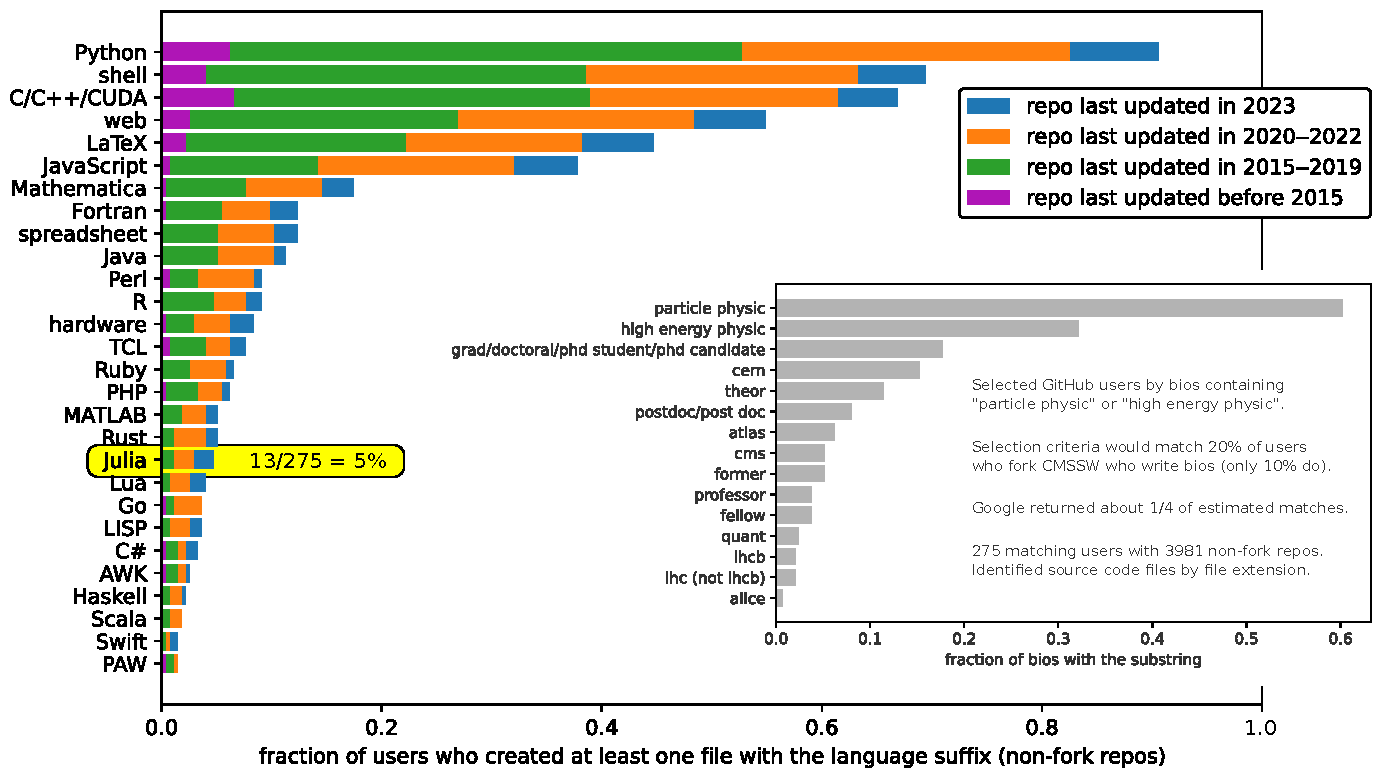
\includegraphics[width=\linewidth]{physicist-languages-presentation.pdf}
\end{frame}

%% "Julia" in Materials, up to a year ago (starting January 2022): 431

%% Removed because author's name is Julia:
%% (+ 1 2 1 1 2 1 1 1 1 6 7 7 7 8 8 7 7 7 7 7 6 7 7 8 8 7 7 8 2 2 4 9 8 8 7 4)
%% 191
%% Documents that reference Julia as a human name:
%% (+ 1 1 1 1 1 1 1 1 1 1 1 1 1 1 1 1 1 1 1 1 1 1 1 1 1 1 1 1 1 1 1 1 1 1 1 1 1 1 1 1 1 1 1 1 1 1 1 1 1 1 1 1 1 1 1 1 1 1 1 1 1 1 1 1 1 1 1 1 1 1 1 1 1 1 1 1 1 1 1 1 1 1 1 1 1 1 1 1 1 1 1 1 1 1 1 1 1 1 1 1 1 1 1 1 1 1 1 1 1 1 1 1 1 1 1 1 1 1 1 1 1 1 1 1 1 1 1 1 1 1 1 1 1)
%% 133
%% Documents that reference Julia the programming language:
%% (+ 1 1 1 1 1 1 1 1 1 1 1 1 1 1 1 1 1 1 1 1 1 1 1 1 1 1 1 1 1 1 1 1 1 1 1 1 1 1 1 1 1 1 1 1 1 1 1 1 1 1 1 1 1 1 1 1 1 1 1 1 1 1 1)
%% 63
%% (1 reference to JULIA (Job to Unveil LEP Interactions in Aleph), 1985-1989)
%% Documents that have no match to "Julia":
%% 1
%% Meaning of "Julia" is other or not clear:
%% 1 1 1

%% "Rust" in Materials, up to a year ago (starting January 2022):

%% Documents that refer to oxidized metal:
%% (+ 1 1 1 1 1 1 1 1 1 1)
%% 10
%% Documents that refer to Rust the programming language:
%% (+ 1 1 1 1 1 1 1 1 1 1 1 1)
%% 12
%% Other/unclear:
%% 1 1 1 

%% "Lua" in Materials, up to a year ago (starting January 2022):

%% Documents that refer to the LHC User's Association:
%% 1 1 1 1

%% Documents that refer to Lua the programming language:
%% 1 (used in SIMION electric field and charge particle simulator)

%% Other/unclear:
%% 1 1 1 1 

\begin{frame}{But physicists are more interested in Julia than, say, Rust or Lua}
\vspace{0.5 cm}
Among ``Materials'' (PDFs and TXTs) in CERN's Indico search since January 2022,

\vspace{0.25 cm}
\begin{description}
\item[\textcolor{darkorange}{\bf 63}] \textcolor{darkorange}{\bf refer to Julia the programming language}
\item[324] refer to people named Julia
\item[4] other/unclear
\end{description}

\begin{description}
\item[\textcolor{darkorange}{\bf 12}] \textcolor{darkorange}{\bf refer to Rust the programming language}

(7 of those same documents also refer to Julia)
\item[10] refer to oxidized metal
\item[3] other/unclear
\end{description}

\begin{description}
\item[\textcolor{darkorange}{\bf 1}] \textcolor{darkorange}{\bf refers to Lua the programming language}

(it's used to configure the SIMION charged particle simulator)
\item[4] refer to the LHC User's Association
\item[4] other/unclear
\end{description}
\end{frame}

%% Julia in CHEP 2023: 3 titles and 4 abstracts
%% 1 1 1 1 

%% Python in CHEP 2023: 1 title and 35 abstracts
%% 1 1 1 1 1 1 1 1 1 1 1 1 1 1 1 1 1 1 1 1 1 1 1 1 1 1 1 1 1 1 1 1 1 1 1 

%% Julia in ACAT 2022: 1 title and 1 abstract
%% Binned histogram fitting for Bayesian inference via Automatic Differentiation in JuliaLang

%% Python in ACAT 2022: 3 titles and 24 abstracts

\begin{frame}{Similarly, it is increasingly a focus on ACAT and CHEP}
\vspace{0.5 cm}

\textcolor{darkblue}{\Large\bf ACAT 2022:}
\begin{itemize}
\item Julia: 1 title and 1 abstract
\item Python: 3 titles and 24 abstracts
\end{itemize}

\vspace{0.5 cm}
\textcolor{darkblue}{\Large\bf CHEP 2023:}
\begin{itemize}
\item Julia: 3 titles and 4 abstracts
\item Python: 1 title and 35 abstracts
\end{itemize}

\vspace{0.5 cm}
Only other programming languages mentioned: C++ (frequently) and Java (2 times).
\end{frame}

\begin{frame}{And, it's the only language-based HSF group other than PyHEP}
\vspace{0.15 cm}
\begin{center}
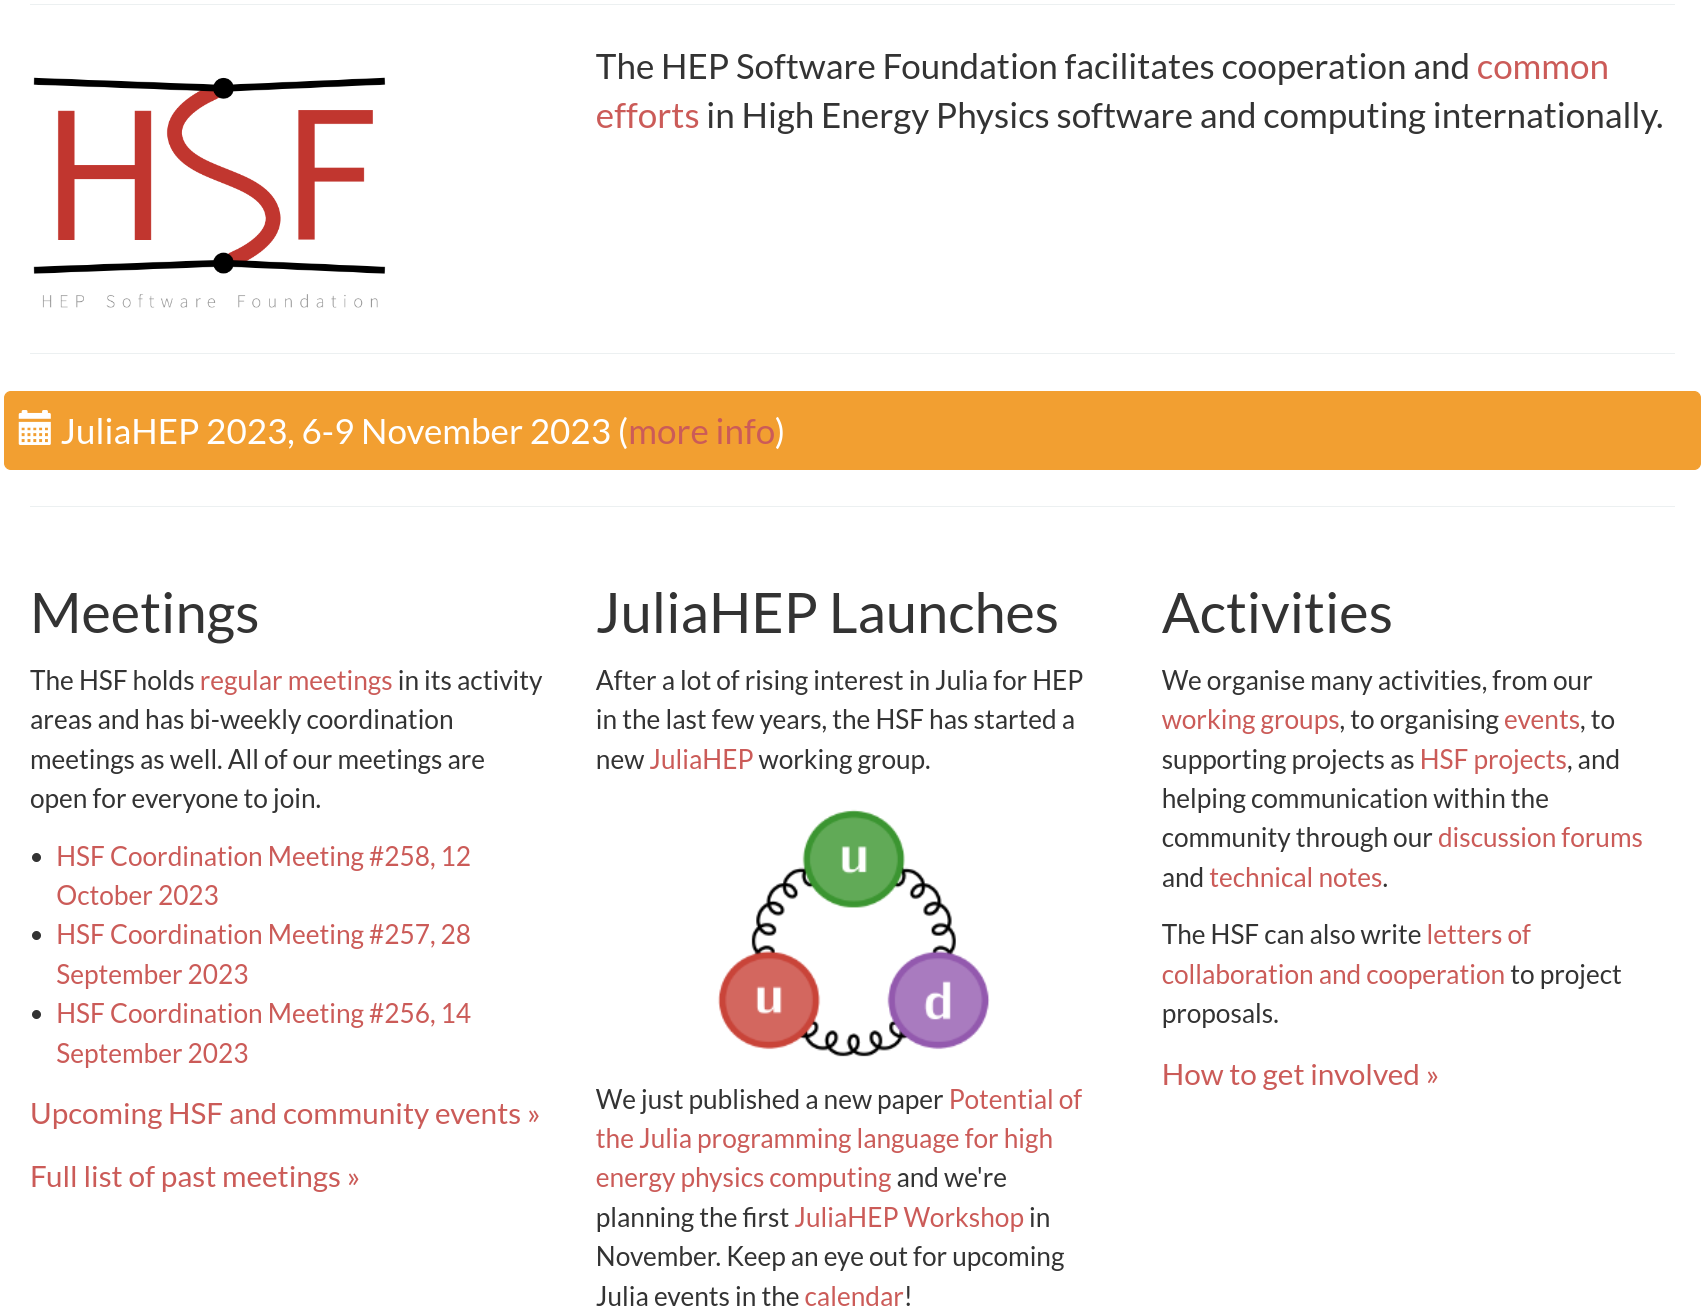
\includegraphics[width=0.72\linewidth]{juliahep-website.png}
\end{center}
\end{frame}

\begin{frame}{\mbox{ }}
\vspace{0.5 cm}
\LARGE
\begin{center}
\textcolor{darkblue}{Julia is not yet ``adopted'' in HEP, but it is getting more attention than any other rival to C++ and Python.}
\end{center}

\vspace{1 cm}
\begin{center}
\uncover<2->{\textcolor{darkblue}{From here, it could continue to rise in prominence \\ or end up being a fad. This is a critical time.}}
\end{center}
\end{frame}

\begin{frame}{\mbox{ }}
\large
\vspace{0.5 cm}
\textcolor{darkblue}{\Large As we've seen, Julia is a perfect fit for HEP, technologically.}

\vspace{0.5 cm}
\begin{itemize}
\item<2-> It allows for an exploratory phase, in which the data analyst focuses on {\it what} to compute, rather than how it will be accelerated.
\item<3-> It allows the exploratory code to be tweaked to scale up to large datasets.
\end{itemize}

\vspace{0.5 cm}
\uncover<4->{There is a {\it gradual path} from brainstorming to optimized code.}
\end{frame}

\begin{frame}{\mbox{ }}
\vspace{0.5 cm}
\large
\begin{center}
This argument focuses on Julia as a solution to the two-language problem, but we can't go from two languages to one language without going through three.
\end{center}

\vspace{0.25 cm}
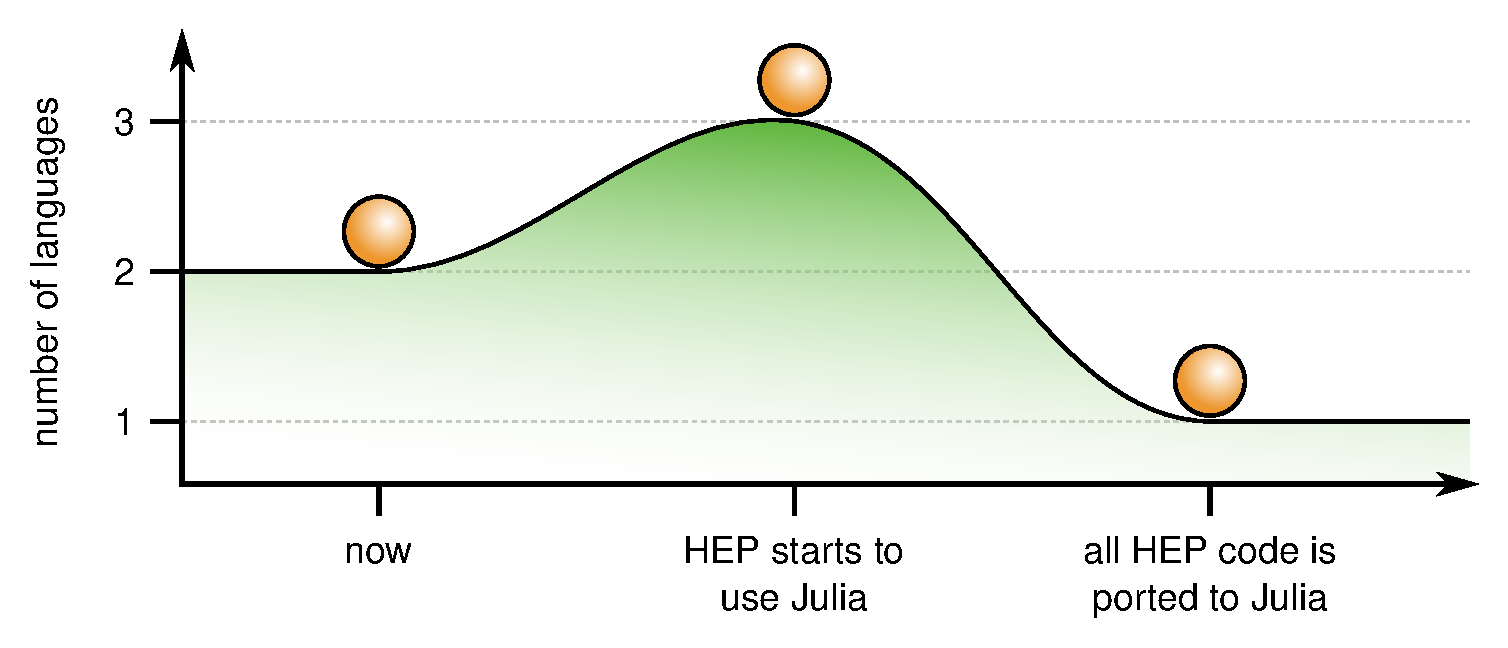
\includegraphics[width=\linewidth]{number-of-languages.pdf}
\end{frame}

\begin{frame}{\sout{``If you build it, they will come.''}}
%% \vspace{-1.55 cm}
%% \hspace{6.5 cm}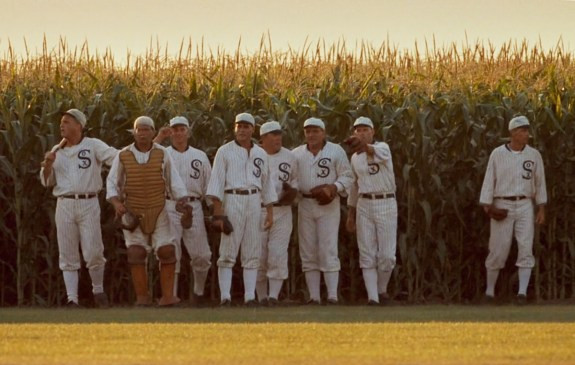
\includegraphics[height=1 cm]{field-of-dreams.jpg}
%% \vspace{1 cm}

\Large
\vspace{0.6 cm}
Preparing a complete stack of HEP tools in Julia will help adoption, but it will not eliminate the interim 3-language period.

\vspace{0.95 cm}
\uncover<2->{There will not be any clean break in which everyone is ready to set aside their old tools and take up new ones.}

\large
\vspace{0.95 cm}
\uncover<3->{\textcolor{darkgrey}{(The closest approximation to that in HEP was the Fortran $\to$ C++ transition, which was mandated top-down and lost a generation of HEP programmers.)}}
\end{frame}

\begin{frame}{}



\end{frame}


\end{document}
